\input{wsc17style.tex}

\documentclass{wscpaperproc}

\usepackage{latexsym}
\usepackage{caption}
\usepackage{graphicx}
\usepackage{subcaption}
\usepackage[utf8]{inputenc}
\usepackage[table]{xcolor}
\usepackage{graphicx}

\begin{document}

\WSCpagesetup{Ortega and Salgado}

\title{QUEUE ANALYSIS FOR A SUPERCOMPUTING CENTER}

\author{Andrés Felipe Ortega Montoya\\ [12pt]
aortega7@eafit.edu.co\\
Ingeniería Matemática\\
Universidad EAFIT\\
\and
Alejandro Salgado Gómez\\[12pt]
asalgad2@eafit.edu.co\\
Ingeniería Matemática\\
Universidad EAFIT\\
}

\maketitle

\section{Conceptual modeling}

\subsection{Problem definition}

The growth of data and problem sizes in the last couple of years has
triggered an unprecedented increase in the need of computational
power. This need has induced a boost in the utilization of
elements like supercomputers.

Because of this, the computing centers are experimenting an unprecedented growth
in the amount of tasks to process. Thus the problem of resource assignation has
become an issue of great importance for this type of systems in order to
provide a good service and achieve a better use of their resources. However due
to the varied amount of time each of the jobs can take to compute, it
constitute a problem to provide a reasonable waiting time to all users.

For this reason the ideas and solutions that the discrete simulation can provide
are specially useful for this type of establishments, mainly because of
the improvements that can be made in terms of attention time and resource
utilization.

\subsection{Objectives}

\subsubsection{Model purpose}

The current model aims to present a simplified version of a real supercomputing
system in order to analyse its behavior. The main intention is to understand
which possible set of causes explains the principal waiting times and, if
possible, determine modifications that can improve the service for most
of the user population.

\subsubsection{Specific objectives}

\begin{itemize}
    \item Have a first hand approach to the process of create a descrete event
          model of a real system.
    \item Use a descrete event model to better understand the process that
          characterized a supercomputer.
    \item Analyze the behavior at each step of the process in the system.
    \item If possible, suggest ideas to optimize the performance of the actual
          system.
\end{itemize}

\subsubsection{Project objective}

This project aims to model the Scientific Computing Center APOLO as a
discrete event simulation. The main objective is to experiment the
application of the theory addressed in the course by working with a real
system. The intention is to analyze the occupation process of the
supercomputer and if it is possible, suggest alternatives to improve
the performance of the computing center in terms of attention to users
and resource utilization.

\subsection{Inputs and outputs}

\subsubsection{Inputs}

\begin{itemize}
    \item
\end{itemize}

\subsubsection{Outputs}

\begin{itemize}
    \item Average time in queue.
    \item Average time in the system.
    \item Number of jobs completed.
    \item utilization and idle percentages from both queues and nodes.
\end{itemize}

\subsection{Contents}

\subsubsection{Scope}

This project aims to simulate the three main queues of the Cientific Computing
Center APOLO as a discrete event model. Data from the three months with a higher
usage were selected to feed the model. The main purpose is not to use the model
to improve the system but to have a first hand approach to the modeling process
of a real system by appliyng the knowledge acquired in the class.

\subsubsection{Detail level}

The model only considers the three main queues of APOLO. Each of the queues are
modeled independently and their jobs are classified based on the time they
expend doing computations (seconds, minutes, hours or days).  Each job can
represent a group of similar jobs. All computing nodes from the Computing
Center are taken into account, but nodes are taken as composed exclusively by
CPUs, other hardware is not taken into account.

\subsubsection{Assumptions}

\begin{itemize}
    \item The number of arrivals per hour is taken as a poisson process.
    \item Each queue is independent to manage their jobs.
    \item Jobs label as failed have a execution time of 0.
\end{itemize}

\subsubsection{Simplifications}

\begin{itemize}
    \item Only the three main queues of APOLO are taken into account.
    \item Groups of jobs are taken as a single job with a higher execution time.
    \item Queues are assume to be empty at the begining of the simulation.
    \item Only CPUs are taken into account as resources.
\end{itemize}

\section{State of the art}

This type of project is not new, in \cite{article1} there is an implementation
of a discrete event simulation model to analyse how the horizontal scaling
influence the performance of the a cloud computing system. In this work the main
objective was to explore the relationship between the horizontal scaling
profile configurations and the functionality of the cloud model. In
\cite{article2} there is an implementation that uses queue theory to study the
quality of service in a cloud computing system, in order to search for
configurations that allows a good service and a commercial success. Finally in
\cite{article3} there is an implementation that aims to model
the interarrival time and service time distributions of a MPP system (Massively
Parallel Processor). In this paper they describe the process as
dispersive and complex due to the specific distributions they have to use, such
as a Hyper Erlang distribution.

\section{Data}

APOLO has slurm \cite{slurm} as resource manager, which means that slurm is in
charge of control the assignation of resources that each job needs. This program
works by mange queues where jobs wait for their resources to be released in
order to start their excecution. This program stores all the information related
to the resource management in a relational database, which allows an easy
access to the information about the cluster utilization.\\

The allocation process is splited in three main queues. They are
\begin{itemize}
    \item \textbf{longjobs:} queue for jobs that are intensive in the use of CPU.
    \item \textbf{accel:} queue for jobs that use GPU computation.
    \item \textbf{bigmem:} queue for jobs that use large amount of memory.
\end{itemize}

The data used in this work comes from jobs that were either waiting or executing
at the supercomputer from May to July of 2017, which are the months with higher
demand of resources in that year. A sample of this data looks like
this

\begin{itemize}
    \item \textbf{JobID:} 44256
    \item \textbf{AllocCPUS:} 32
    \item \textbf{State:} COMPLETED
    \item \textbf{Submit:} 2017-04-27T05:42:00
    \item \textbf{Start:} 2017-05-02T07:59:01
    \item \textbf{Elapsed:} 1-09:26:13
    \item \textbf{End:} 2017-05-03T17:25:14
    \item \textbf{Partition:} longjobs
\end{itemize}

This data was used to estimate two main groups of distributions and parameters,
the ones related to interarrival time of jobs and the ones related to execution
time, both for each queue.

In the case of the interarrival time the information that is needed is the
number of jobs per hour. This in order to estimate the parameter of an
exponential distribution as 1 over the number of jobs per hour, since the
process of arrivales is taken as described by a poisson distribution.
The results are shown in Figures \ref{arrival_longjobs}, \ref{arrival_accel} and
\ref{arrival_bigmem}.

\begin{figure}[h!]
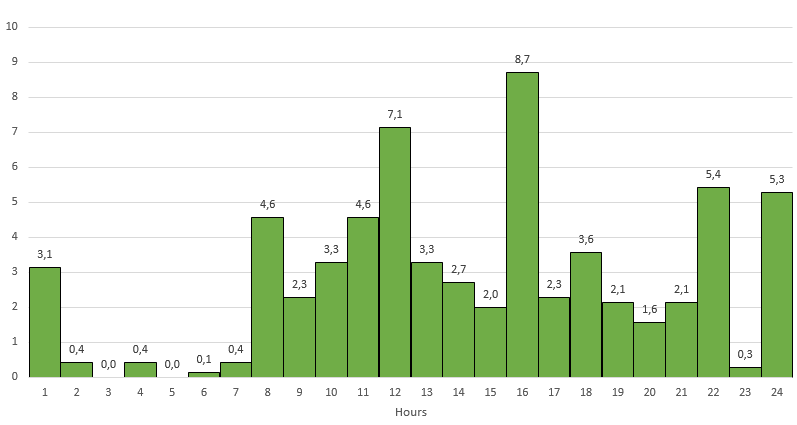
\includegraphics[width=\textwidth]{./images/average_arrivals_longjobs}
\caption{Average number of jobs per hour (longjobs)}
\label{arrival_longjobs}
\end{figure}

\begin{figure}[h!]
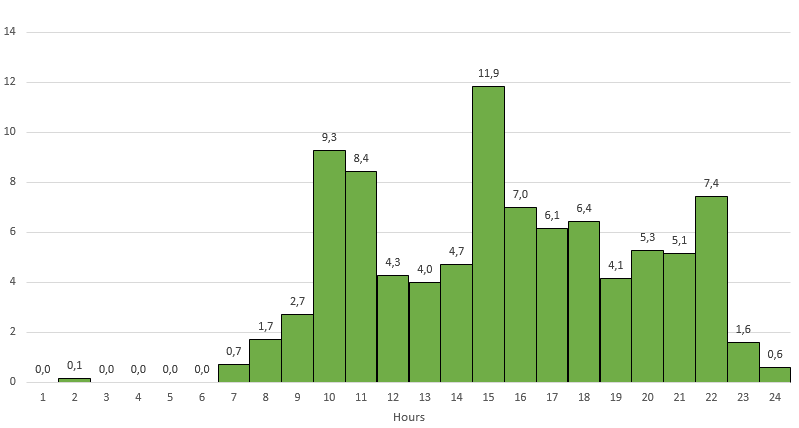
\includegraphics[width=\textwidth]{./images/average_arrivals_accel}
\caption{Average number of jobs per hour (accel)}
\label{arrival_accel}
\end{figure}

\begin{figure}[h!]
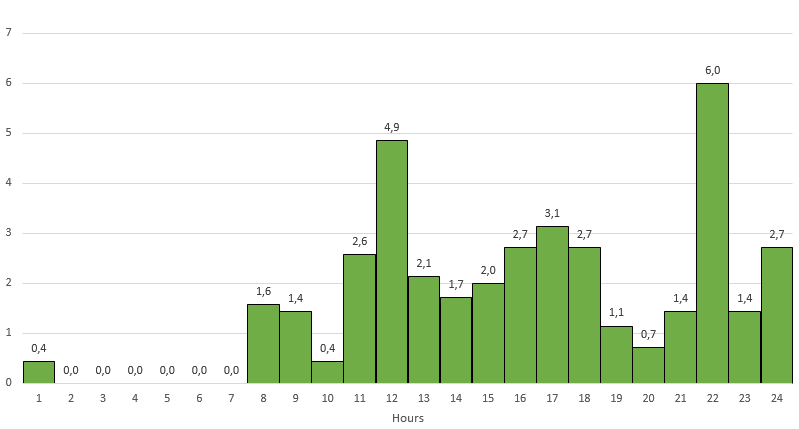
\includegraphics[width=\textwidth]{./images/average_arrivals_bigmem}
\caption{Average number of jobs per hour (bigmem)}
\label{arrival_bigmem}
\end{figure}

Finally it was found that the execution time of jobs could be represented with
probability distributions. This because of the sparce autocorrelation plots that
results when groups of jobs submited at the same time and
whith similar requests of resources are joined in a single job with higher
execution time. With this in mind a kolmogorov smirnov test was conducted to
estimate the distributions. \\

Its important to highlight that the execution time varies from seconds to days,
so analysis of the process was splited in order to work with samples in the same
units of time. The division consists in work with jobs in the following ranges
of time

\begin{itemize}
    \item 1 to 60 seconds
    \item 1 to 60 minutes
    \item 1 to 24 hours
    \item 1 to the maximum number of days that a job can use
\end{itemize}

The results are shown in Tables \ref{distributions_longjobs},
\ref{distributions_accel} and \ref{distributions_bigmem}.

\begin{table}[h!]
    \centering
    \begin{tabular}{ | c | c | c | c |}
        \hline
        \textbf{Time unit} & \textbf{distribution} & \textbf{parameters} & \textbf{p-value} \\
        \hline
        Seconds & Uniform & a=1, b=56 & 0.88 \\
        \hline
        Minutes & Beta & $\alpha_1$=1.3, $\alpha_2$=11.2, min=0, max=83.3 & 0.82 \\
        \hline
        Hours & Beta & $\alpha_1$=1.28, $\alpha_2$=1.61, min=0, max=23.4 & 0.76 \\
        \hline
        Days & Empirical & N/A & N/A \\
        \hline
    \end{tabular}
    \caption{Execution time distributions (longjobs)}
    \label{distributions_longjobs}
\end{table}

\begin{table}[h!]
    \centering
    \begin{tabular}{ | c | c | c | c |}
        \hline
        \textbf{Time unit} & \textbf{distribution} & \textbf{parameters} & \textbf{p-value} \\
        \hline
        Seconds & Empirical & N/A & N/A \\
        \hline
        Minutes & Empirical & N/A & N/A \\
        \hline
        Hours & Empirical & N/A & N/A \\
        \hline
        Days & Gamma & $\alpha$=0.94, $\beta$=1.87 & 0.95 \\
        \hline
    \end{tabular}
    \caption{Execution time distributions (accel)}
    \label{distributions_accel}
\end{table}

\begin{table}[h!]
    \centering
    \begin{tabular}{ | c | c | c | c |}
        \hline
        \textbf{Time unit} & \textbf{distribution} & \textbf{parameters} & \textbf{p-value} \\
        \hline
        Seconds & Uniform & a=1, b=60 & 7.6 \\
        \hline
        Minutes & Gamma & $\alpha$=0.7, $\beta$=18.2 & 0.73 \\
        \hline
        Hours & Gamma & $\alpha$=0.91, $\beta$=6.99 & 0.66 \\
        \hline
        Days & Gamma & $\alpha$=2.24, $\beta$=1.01 & 0.941 \\
        \hline
    \end{tabular}
    \caption{Execution time distributions (bigmem)}
    \label{distributions_bigmem}
\end{table}

\section{Implementation}

\section{Verification and validation}

\section{Experimentation}

\subsection{Results}

\subsubsection{model nature} Salvaje y despiadado (Solo quiere ver el mundo arder)
\subsubsection{Output nature}
\subsubsection{Initial bias}
\subsubsection{Number of executions}
\subsubsection{Solution space}

\subsection{Sensitivity analysis}

\section{Conclusions}

\begin{itemize}
    \item This model is awesome!
\end{itemize}

\bibliographystyle{wsc}
\bibliography{entrega2}

\end{document}
